\documentclass{article}


\usepackage{graphicx}
\usepackage{amsmath}
\usepackage{amssymb}



\newtheorem{theorem}{Theorem}

\title{From Mass-Spring Systems to Spectral Graph Neural Networks}
\author{Nguyen Ngoc Khanh}

\begin{document}
    \maketitle

    \section{Mass-Spring System}

    \subsection{The two particles system}

    Consider a spring follows Hook's law. Let two particles $i$ and $j$ connected by a spring located at $x_i$ and $x_j$ respectively and $e_{i j} = \frac{x_j - x_i}{||x_j - x_i||_2}$ be the direction from $x_i$ to $x_j$ then the force that $i$ affects $j$ can be represented as:

    \begin{equation}
        F_{i j} = - k (||x_j - x_i)||_2 - L) e_{i j} = - k (x_j - x_i) + k L e_{i j}
    \end{equation}

    where $k$ is a positive real number, the characteristic of the spring and $L$ is the initial length the of spring. The magnitude of the force is proportional to the displacement from the initial distance between two particles.

    Let two particles connected by a spring sit in an Euclidean space such that the particles can freely move on a particular $z$ axis. At the initial condition, the two particles are located at $x_i$ and $x_j$ and the spring is at its length ($||x_j - x_i||_2 = L$) (no force).

    \begin{figure}[h!]
        \centering
        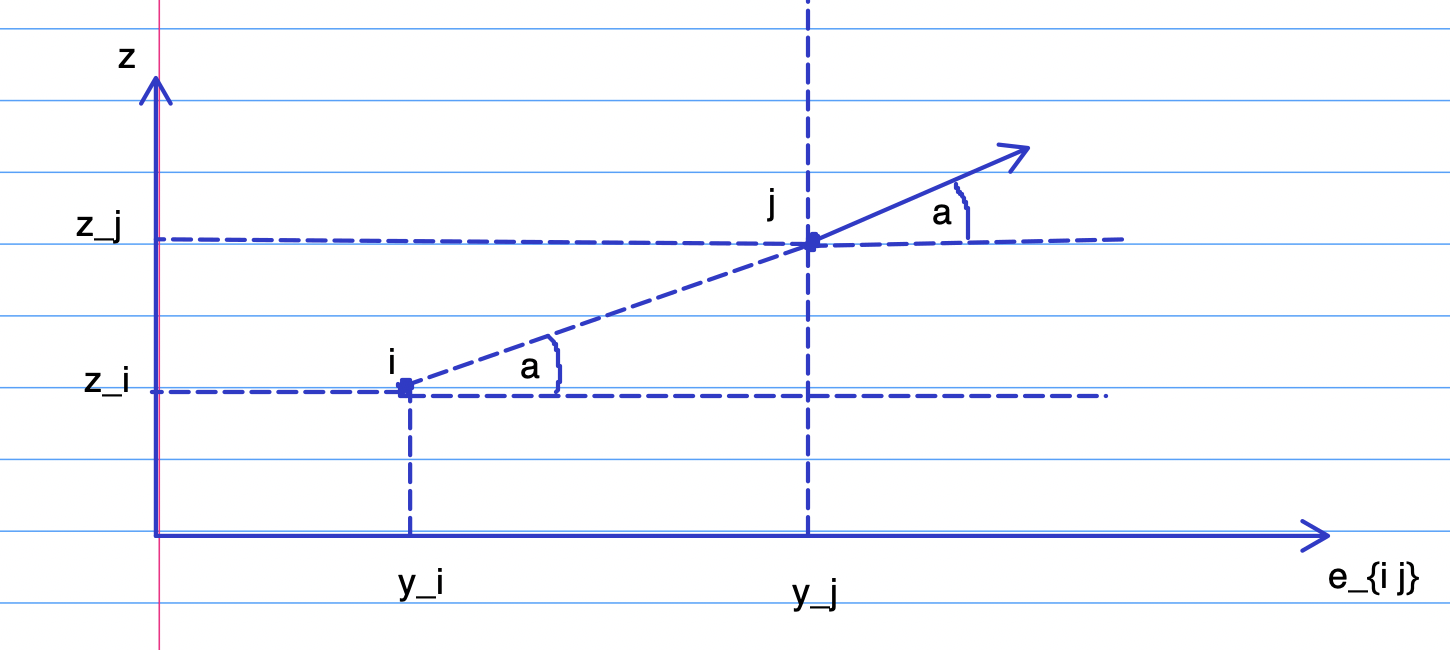
\includegraphics[width=0.8\textwidth]{fig1.png}
        \caption{subspace of $e_{i j}$ and $z$}
        \label{fig:fig1}
    \end{figure}

    Since, $i$ and $j$ can only move in the $z$ axis, we can rewrite

    \begin{gather*}
        x_i = x_i^{(0)} + z_i z \\
        x_j = x_j^{(0)} + z_j z \\
    \end{gather*}

    Where $x_i^{(0)}$ and $x_j^{(0)}$ are the initial positions of $i$ and $j$, $z_i$ and $z_j$ are the displacements on the $z$ axis. Hence, the projected force on the $z$ axis can be written as

    \begin{equation}
        F_{i j} \cdot z = (- k (x_j - x_i) + k L e_{i j}) \cdot z = (- k (x_j^{(0)} - x_i^{(0)}) + k L e_{i j}) \cdot z + (- k (z_j - z_i) z) \cdot z
    \end{equation}

    The first term is the dot product of the initial force with the $z$ direction which is essential zero since there is no force at the beginning. Hence, the projected force on the $z$ axis can be written as

    \begin{equation}
        F_{i j} \cdot z = - k (z_j - z_i)
    \end{equation}

    The projected force on the $z$ axis linearly depends on the corresponding displacement.

    \subsection{The n particles system}

    Let $n$ particles with the same weight $m$ on an an Euclidean space that can freely move on a particular $z$ axis. Some of them are connected by springs of the same characteristic $k$ which is denoted by a undirected unweighted graph $G = (V, E)$. A particular node $i$ is affected by all of its neighbours where the projected force on $i$ is

    \begin{figure}[h!]
        \centering
        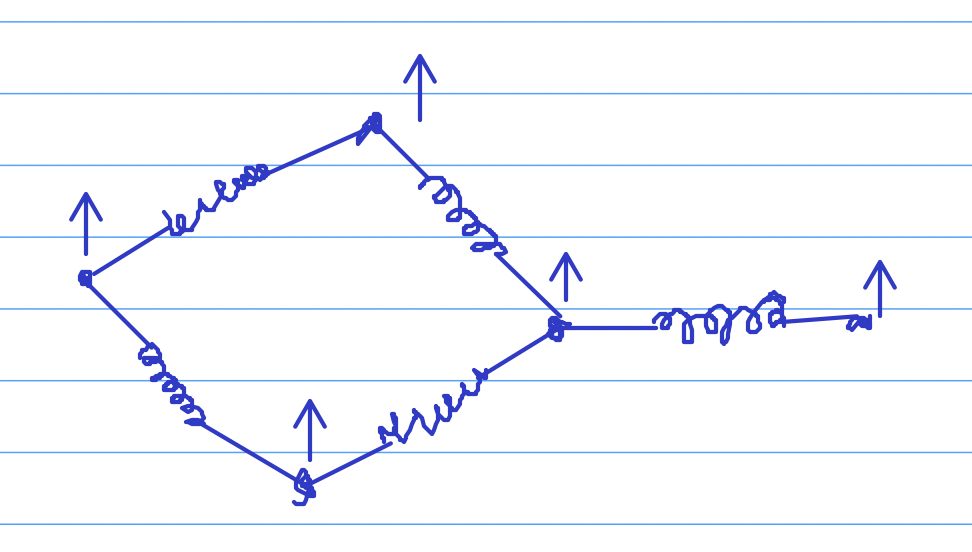
\includegraphics[width=0.8\textwidth]{fig2.png}
        \caption{4 particles system}
        \label{fig:fig2}
    \end{figure}

    \begin{equation}
        F_i \cdot z = - k \sum_{e_{j i} \in E} z_i - z_j = - k (d_i z_i - \sum_{e_{j i} \in E} z_j)
    \end{equation}

    Where $d_i$ denotes the degree of the node $i$. Newton's Second Law of Motion:

    \begin{gather*}
        a_i \cdot z = \frac{F_i}{m} \cdot z \\
        \ddot{z_i} = - \frac{k}{m} (d_i z_i - \sum_{e_{j i} \in E} z_j)
    \end{gather*}

    We can rewrite in the matrix form

    \begin{equation}
        \ddot{z} =  - \frac{k}{m} (D - A) z = - \frac{k}{m} L z
        \label{eq:newton_2nd}
    \end{equation}

    Where $z = (z_1, z_2, ..., z_n)^T$, $A$ is the adjacency matrix of $G$ and $D$ is the degree matrix of $A$ (diagonal matrix where each entry equals to the corresponding degree of the node). $L = D - A$ is called Laplacian matrix of $A$.

    We are seeking the mode of oscillation of the system. A mode of oscillation is a particular frequency where all particles oscillate at the same frequency. At that frequency, the differential equation for each particle must be in the form:

    \begin{equation}
        \ddot{z_i} = - \omega^2 z_i
    \end{equation}

    Where $\omega$ is the frequency. In the matrix form:

    \begin{equation}
        \ddot{z} = - \omega^2 z
        \label{eq:oscillation_mode}
    \end{equation}

    From \ref{eq:newton_2nd} and \ref{eq:oscillation_mode}, we have

    \begin{equation}
        L z = \frac{m}{k} \omega^2 z
        \label{eq:oscillation_mode_freq}
    \end{equation}

    From \ref{eq:oscillation_mode_freq}, the oscillation mode frequencies are equivalent to the eigenvalues of the Laplacian matrix, and the initial condition to achieve each of the frequencies is the corresponding eigenvector.

    Since $L$ is real symmetric, by the Spectral Theorem, it has an eigenbasis. Furthermore, $L$ is positive semi definite, then all of its eigenvalues are positive, hence the frequencies make sense.

    For an arbitrary initial condition, since the system is linear, we can decompose the displacement $z$ into the eigenbasis of the Laplacian matrix then solve each of the component individually.

    \section{Graph Laplacian Basis}

    Recall that, the eigen decomposition of $L$ is as follow:

    \begin{equation}
        L = U \Lambda U^T = U \Lambda U^{-1}
    \end{equation}

    Where each column vector in $U$ is a normalized eigenvector.

    Analogous to Fourier Transform, the eigenvalues of Laplacian matrix can serve as the frequency and the eigenbasis is corresponding to the Fourier basis.

    Let $x \in \mathbb{R}^n$ be a graph signal on $G = (V, E)$ where each component of $x$ is a real number corresponding to a node in $G$.

    The convolution in spatial domain is equivalent to multiplication in spectral domain. Define the convolution operation as:

    \begin{equation}
        y(x) =  U ( U^T w \odot U^T x )
        \label{eq:conv_vec}
    \end{equation}

    Where $w \in \mathbb{R}^n$ is called filter or kernel. Define $W = diag(U^T w)$ be the diagonal matrix whose entries are the entries of $U^T w$, we can rewrite \ref{eq:conv_vec} as

    \begin{equation}
        y(x) =  (U W U^T) x
    \end{equation}

    \subsection{ChebNet}


    Let $\mathcal{L}$ be the normalized laplacian matrix.

    \begin{equation}
        \mathcal{L} = D^{-\frac{1}{2}} L D^{-\frac{1}{2}} = I - D^{-\frac{1}{2}} A D^{-\frac{1}{2}}
    \end{equation}

    The decomposition of $\mathcal{L}$

    \begin{equation}
        \mathcal{L} = U \Lambda U^T = U \Lambda U^{-1}
    \end{equation}

    \begin{theorem}(Chung \cite{chung1997spectral})
        All eigenvalues of $\mathcal{L}$ are in the interval $[0, 2]$.
    \end{theorem}

    ChebNet \cite{defferrard2016convolutional} approximate the diagonal matrix $W$ using Chebyshev polynomials as the orthogonal basis in the polynomial subspace of the vector space of all functions $f: [-1, +1] \to \mathbb{R}$ with respect to the inner product.

    \begin{equation}
        \int_{-1}^{+1} f(x) g(x) \frac{dx}{\sqrt{1-x^2}}
    \end{equation}

    Chebyshev polynomials of the first kind:

    \begin{equation}
        T_{n+1}(x) = 2x T_n(x) - T_{n-1}(x)
    \end{equation}

    Where $x \in [-1, +1]$, $T_0(x) = 1$ and $T_1(x) = x$. Let $f_i: [-1, +1] \to \mathbb{R}$ is an arbitrary function such that $f_i(\Tilde{\lambda_i}) = w_i$ where $\Tilde{\lambda_i} = \frac{2 \lambda_i}{\lambda_{\max}} - 1 \in [-1, +1]$, $\lambda_{\max}$ is the largest eigenvalue. We want to project $f_i$ into the subspace with the orthogonal basis of the first $K$ terms of Chebyshev polynomials of the first kind. We can write $f_i$ as

    \begin{equation}
        \hat{f}_i(t) = \sum_{k=0}^{K-1} \theta_{k i} T_k(t)
    \end{equation}

    Hence, $w_i$ is approximated as

    \begin{equation}
        \hat{w_i} = \hat{f}_i(\Tilde{\lambda_i}) = \sum_{k=0}^{K-1} \theta_{k i} T_k(\Tilde{\lambda_i})
    \end{equation}

    Matrix form of the approximation on $W$:

    \begin{equation}
        \hat{W} = \sum_{k=0}^{K-1} \theta_k T_k(\Tilde{\Lambda})
    \end{equation}

    Where $\Tilde{\Lambda}$ is the diagonal matrix of $\Tilde{\lambda_i}$. Moreover,

    \begin{equation}
        U \hat{W} U^T = \sum_{k=0}^{K-1} \theta_k U T_k(\Tilde{\Lambda}) U^T = \sum_{k=0}^{K-1} \theta_k T_k(\Tilde{\mathcal{L}})
    \end{equation}

    Where $\Tilde{\mathcal{L}} = \frac{2 \mathcal{L}}{\lambda_{\max}} - I$. It is a great exercise to prove the Chebyshev recurrence for $\Tilde{\mathcal{L}}$:

    \begin{equation}
        T_{n+1}(\Tilde{\mathcal{L}}) = 2 \Tilde{\mathcal{L}} T_n(\Tilde{\mathcal{L}}) - T_{n-1}(\Tilde{\mathcal{L}})
    \end{equation}



    Finally, The convolution operation is

    \begin{equation}
        y(x) = \sum_{k=0}^{K-1} \theta_k T_k(\Tilde{\mathcal{L}}) x
    \end{equation}

    The construction of ChebNet avoids decomposing the matrix $L$ as compare to \ref{eq:conv_vec}.

    \subsection{Graph Convolutional Network}

    Similar to ChebNet, GCN \cite{kipf2016semi} limits $K = 2$ and sets $\lambda_{\max} = 2$ hence $\Tilde{\mathcal{L}} = \mathcal{L} - I$.

    \begin{gather*}
        U \hat{W} U^T = \theta_0 T_0(\Tilde{\mathcal{L}}) + \theta_1 T_1(\Tilde{\mathcal{L}}) \\
        = \theta_0 I + \theta_1 \Tilde{\mathcal{L}} \\
        = \theta_0 I - \theta_1 D^{-\frac{1}{2}} A D^{-\frac{1}{2}}
    \end{gather*}

    The convolution operation is

    \begin{equation}
        y(x) = \theta_0 x - \theta_1 D^{-\frac{1}{2}} A D^{-\frac{1}{2}} x
    \end{equation}

    The notes here is greatly inspired by \cite{chen2020note}.

    \bibliographystyle{plain}
    \bibliography{references}
\end{document}